\section{一页总览：项目到底在算什么}\label{sec:overview}
\textbf{程序计算一个已给定能量、尺寸和动量分布的电子束团，经过漂移、磁透镜、RF 与空间电荷作用后，怎样到达样品诊断面。}默认参考动能为 100 keV。起点虽叫 \texttt{cathode}，目前只是几何标记，没有完整光电发射、阴极镜像电荷或电子枪加速；终点也没有样品衍射和探测器成像。

两条物理路线并存：AG 用少量统计量描述束团，计算快、便于分析；OCELOT 追踪宏粒子，保留更多分布形状，用 PIC 算空间电荷。\textbf{每个模型各有一套正式 driver}，日常命令行、验证适配和 GUI 共用它；测试层不再另建一套物理实现。
\begin{table}[H]\centering\small
\begin{tabularx}{\linewidth}{P{24mm}YY}\toprule
 & AG & OCELOT \\ \midrule
状态 & 尺寸、包络斜率、配对相空间面积等约化统计量 & 宏粒子的六维过面坐标和电荷权重 \\
输运 & 包络方程、硬边界近轴磁聚焦 & 漂移二阶；磁透镜显式一阶 \\
纵向 RF & 线性协方差变换 & 时间正弦调制 \\
SC & 高斯闭合 F/G；保留椭球选项 & 自由空间、共同参考系的三维准静态 PIC \\
共同输出 & \multicolumn{2}{p{11cm}}{JSON：束宽、束长、chirp、动量展宽、三方向发射度、时宽及实际位置/溯源；GUI 展示、比较和导出。} \\
\bottomrule\end{tabularx}
\caption{共享问题与数据约定，不代表两种近似在所有物理量上等价。}
\end{table}

AG 已补齐 Gx/Gy/Gz，发射度不再一律固定，但不能恢复所有非高斯高阶关联。OCELOT 也不是绝对真值：网格、宏粒子、步长、随机抽样、一阶磁透镜和准静态假设都限制精度。

GUI 已实现参数与位置编辑、几何预检、运行/停止、曲线和导出。Windows 兼容代码已加入，并在本轮修复退出与监控错误路径；现有证据是 macOS 上的回归与模拟 Windows 分支测试，\textbf{Windows 实机验收仍未完成}。
\source{\coderef{entry}、\coderef{worker}；物理 Notes；当前数值研究\ev{E08}；GUI/平台日志\ev{E09}、\ev{E10}。}

\clearpage
\section{代码架构与真实调用路径}\label{sec:architecture}
\subsection{四层职责与调用图}
\begin{figure}[H]\centering
\begin{tikzpicture}[>=Latex,
 box/.style={draw=accent!55,rounded corners=1mm,fill=pale,align=center,font=\small,minimum height=12mm},
 arr/.style={->,draw=accent,line width=.7pt}]
\node[box,text width=13.4cm] (in) at (0,0) {共享 YAML 或 GUI 冻结配置\\常量、参考粒子、坐标、开关、几何与输出约定};
\node[box,text width=6.2cm] (ag) at (-3.55,-1.9) {AG：CLI / 验证 / GUI worker\\\texttt{AG.runner.run\_from\_config}};
\node[box,text width=6.2cm] (oc) at (3.55,-1.9) {OCELOT：CLI / 验证 / GUI worker\\\texttt{ued\_beamline\_v2.run\_from\_config}};
\node[box,text width=6.2cm] (ac) at (-3.55,-3.7) {初态、磁场、RF 入口分段\\\texttt{propagate} $\to$ RHS / F / G / $\alpha$};
\node[box,text width=6.2cm] (pc) at (3.55,-3.7) {builder、粒子生成、正式追踪\\活动映射 + 原生 SC + RF 事件};
\node[box,text width=13.4cm] (out) at (0,-5.6) {共同诊断与保存：\texttt{BeamResult / output\_schema}\\JSON、真实事件/覆盖/参考量 $\to$ 比较脚本、GUI 曲线和下载};
\draw[arr] (in.south)-|(ag.north);\draw[arr] (in.south)-|(oc.north);
\draw[arr] (ag)--(ac);\draw[arr] (oc)--(pc);
\draw[arr] (ac.south)--(ac.south|-out.north);\draw[arr] (pc.south)--(pc.south|-out.north);
\end{tikzpicture}
\caption{当前正式数据流。验证层组织案例和判断，不另写追踪循环。}
\end{figure}

\begin{longtable}{P{25mm}P{58mm}P{67mm}}
\toprule 层/目录 & 核心文件 & 责任 \\ \midrule\endhead
共享输入 & \path{shared/params.py}、\path{geometry.py}、\path{run_contract.py} & 参数派生、连续几何检查、显式参数优先级；不复制 SC 力。\\
共享物理边界 & \path{beam_physics.py}、\path{ocelot_coords.py}、\path{rf_model.py} & 参考粒子、原生坐标访问、共同 RF 系数及正弦调制。\\
共同结果 & \path{diagnostics.py}、\path{beam_result.py}、\path{output_schema.py} & 中心矩、派生量、采样查询和统一保存。\\
AG & \path{AG/runner.py}、\path{beam_dynamics_6d.py}、\path{external_forces.py}、\path{alpha_coefficients.py} & driver 管初态/组装/事件；核心管包络、F/G、系数与积分。\\
OCELOT & \path{GPT模拟/ued_beamline_v2.py} & builder、初态、活动映射、Navigator、RF、SC 契约和诊断。\\
验证 & \path{validation/backend.py}、\path{run_all.py}、\path{test_*.py} & 适配正式 driver、独立参考、工程与回归专项。\\
GUI & \path{gui/server.py}、\path{worker.py}、\path{web/} & 本地网页、工作配置、串行任务、进度、图与下载。\\
平台 & \path{gui/platform_compat.py}、根目录启动器 & 子进程、停止、父进程探测和 UTF-8；不改变物理。\\
\bottomrule\end{longtable}

\subsection{入口汇合与仍有的维护成本}
AG CLI \path{AG/run_shared.py} 与 \path{validation.backend.run_ag} 都调用 \path{AG.runner.run_from_config}。OCELOT CLI 与 \path{validation.backend.run_ocelot} 都进入同一个 \path{run_from_config}，再调用 builder/\path{run_beamline}。GUI 同样调用这两套正式实现。

“两路线并行”指两种物理思路并存；GUI 目前\textbf{顺序执行}所选任务，以控制 CPU/内存和停止行为。OCELOT 仍可沿用旧文件名 \texttt{GPT\_results.json}；GPT 只是历史路线标签，不是让语言模型计算粒子。

正式路径已合并，但尚未完全模块化：AG 保留平级导入/\texttt{sys.path} 兼容，GUI 通过只读包装器观察真实进度，OCELOT 主文件同时负责组装、追踪和诊断。这些是维护成本；文件长本身不是物理错误证据。

协方差原型、AG-prime、\path{GPT模拟/bug/} 和分节 benchmark 不自动视为正式替代路线。旧 Windows/MFC 硬件控制工程不属于本束流物理验收，也不应由 GUI 自动运行。
\source{当前正式 driver、\path{validation/backend.py}、\path{AGENTS.md} 第 3 节；\coderef{worker}。}

\section{输入、坐标与输出契约}\label{sec:contracts}
\subsection{默认参数与配置优先级}
共享 YAML 是\textbf{默认名义配置}；GUI 每次任务另存不可变 JSON/YAML 快照。显式 API 参数优先于配置，省略的 SC 参数继承配置。即使配置哈希相同，也须检查有效覆盖、开关和实际方法元数据。
\begin{longtable}{P{52mm}P{25mm}P{73mm}}
\toprule 输入键 & 默认值/单位 & 含义 \\ \midrule\endhead
\path{beam.energy_keV} & 100 keV & 参考动能 $K_0$；OCELOT 生成器接收总能量 GeV。\\
\path{beam.charge_fC} & 100 fC & 物理电荷幅值；AG $N_e=|Q|/e\approx6.24\times10^5$。\\
\path{beam.n_particles} & 50000 & 宏粒子数，控制数值分辨率，不是实际电子数。\\
\path{spot_rms_um} & 85 $\mu$m & 初始 x/y RMS 尺寸，默认圆束。\\
\path{bunch_length_um} & 300 $\mu$m & 束内纵向 RMS 长度。\\
\path{epsilon_n_mm_mrad} & 0.08 $\mmemit$ & 横向归一化 RMS 发射度；乘 $10^{-6}$ 转为 m。\\
\path{sigma_delta} & $10^{-4}$ & $\Delta p/p_0$ 的 RMS，不是 $\Delta E/E_0$。\\
\path{space_charge.enabled} & false & 默认 SC 关；开启后检查 effective 与真实覆盖。\\
\path{space_charge.mesh / step} & $63^3$ / 1 & PIC 网格与过程调度参数，不是 AG 形状参数。\\
\path{output.step_size_m} & 0.005 m & OCELOT 数值设置，不是 AG 自适应内部步长。\\
\path{random.seed} & 42 & 位置 seed，动量重采 seed+1；复现不等于收敛。\\
\path{frequency_GHz} & 2.856 GHz & RF 有效模型频率，可调。\\
\path{voltage_kV / phase_rad} & 30 kV / 3.1416 & 有效积分电压与项目相位，非已标定设备读数。\\
\path{z_start / length} & m & 元件入口/占长；GUI 用 mm 编辑后转为 m。\\
\path{z_diagnostics_mm} & mm 列表 & 名义诊断面，需核对实际位置和方法。\\
\bottomrule\end{longtable}

纵向初始发射度由共享 $\sigma_\zeta,\sigma_\delta$ 和默认零相关推导，不再独立输入。旧 \texttt{epsilon\_nz\_mm\_mrad} 已从默认 YAML 删除；旧配置读取时警告并忽略，避免同一束团被初始化成两种面积。

\subsection{三种纵向量不要混淆}
\begin{equation}
 E_0=K_0+mc^2,\quad\gamma_0=E_0/(mc^2),\quad
 \beta_0=\sqrt{1-\gamma_0^{-2}},\quad p_0=mc\beta_0\gamma_0.
\end{equation}
100 keV 时 $\gamma\approx1.1957$、$\beta\approx0.5482$，不能用 $\beta=1$ 替代。
\begin{align}
 s&:\text{束线位置 [m]}, &\tau&=c\Delta t\quad\text{[m]},\\
 \zeta&=-\beta_0\tau\quad\text{[m，朝束头为正]},
 &\delta_p&=\Delta p/p_0,\\
 q&=p_{\rm oc}=\Delta E/(cp_0), &q&\simeq\beta_0\delta_p.
\end{align}
最后一个关系是一阶、近轴、窄动量展宽适配，不是强能散时的精确运动学。原生 $a=p_x/p_0,b=p_y/p_0$ 也只在近轴范围近似几何斜率。AG 的 \texttt{Beam6D.p0} 却是无量纲 $\beta\gamma$，本文另记 $\bar p_0$，不能拿它当 SI 动量。
\source{官方坐标\cite{occoord}；\path{shared/beam_physics.py}、\path{ocelot_coords.py}；共同诊断 Note。}

\subsection{共同诊断与 JSON 字段}
所有矩先去质心。粒子侧按 $|q_i|$ 作总体权重；零电荷云用等权，不用 $N-1$ 分母。
\begin{equation}
 A=\operatorname{Var}(\zeta),\quad B=\operatorname{Var}(\delta_p),\quad
 C=\operatorname{Cov}(\zeta,\delta_p),\quad D=AB-C^2\ge0.
 \label{eq:cov}
\end{equation}
\begin{equation}
 h=C/A,\quad\varepsilon_{n,p}=\beta\gamma\sqrt D,\quad
 \varepsilon_{\zeta,\zeta'}=\sqrt D/\gamma^2,\quad
 \sigma_t=\sqrt A/(\beta c).
 \label{eq:diag}
\end{equation}
$h$ 是束团实际 chirp，RF 输入 $H$ 是增量斜率；两者不同。纵向 $\varepsilon_{n,p}$ 是本项目的动量坐标归一化面积，“mrad”是报告单位约定，不是真实纵向空间夹角。默认初态 RMS 时宽约 1.83 ps，不能当成整个仪器时间分辨率。
\begin{longtable}{P{53mm}P{24mm}P{73mm}}
\toprule 字段 & 单位 & 读法 \\ \midrule\endhead
\path{z_mm} & mm & 历史实际 $s$；探针还有 nominal/actual/exact。\\
\path{sigma_x_um / sigma_y_um / sigma_z_um} & $\mu$m & 三方向中心化 RMS 尺寸。\\
\path{sigma_delta_e3} & $10^{-3}$ & 字段值乘 $10^{-3}$ 得 $\sigma_\delta$。\\
\path{C_zdelta_m / chirp_per_m} & m / m$^{-1}$ & $C$ 与 $h=C/A$。\\
\path{eps_nx_mm_mrad / eps_ny_mm_mrad} & $\mmemit$ & 横向投影归一化 RMS 发射度。\\
\path{eps_nz_mm_mrad} & $\mmemit$ & $\beta\gamma\sqrt D$ 乘 $10^6$。\\
\path{eps_z_zprime_m} & m & $\sqrt D/\gamma^2$，不可与上项混用。\\
\path{sigma_t_fs} & fs & RMS 时宽。\\
\path{energy_keV / beta_ref / gamma_ref} & keV / 1 / 1 & 各点实际采用的参考量。\\
\path{meta.geometry / rf_events / sc_*} & 以 m 为主 & 几何、RF 实际事件、SC 请求/有效/次数/覆盖。\\
\bottomrule\end{longtable}
AG 非节点探针先插值协方差再求派生量；OCELOT 通常取越过名义面的真实步末状态。比较前先对齐实际面和 RF 前/后事件侧，不能只看标签相同。
\source{\coderef{diagnostic}；\path{shared/beam_result.py}、\path{output_schema.py}；共同诊断 v2 Note。}

\section{元件怎样改变束团}\label{sec:physics}
\subsection{先理解发射度与 chirp}
尺寸回答“多大”，展宽回答“粒子动量差多少”。如果头慢尾快，束团可能在后续漂移中压缩。chirp 是线性位置--动量相关的斜率；发射度描述线性相关解释不掉的厚度：
\begin{equation}
 R=\delta_p-h\zeta,\qquad D=A\operatorname{Var}(R),\qquad h=C/A.
 \label{eq:residual}
\end{equation}
所以大展宽不一定意味着不能压缩；它可能主要是可补偿的 chirp。尺寸与总展宽接近也不保证面积接近：强相关时 $AB-C^2$ 是大数相消，对小关联差异敏感。
\begin{figure}[H]\centering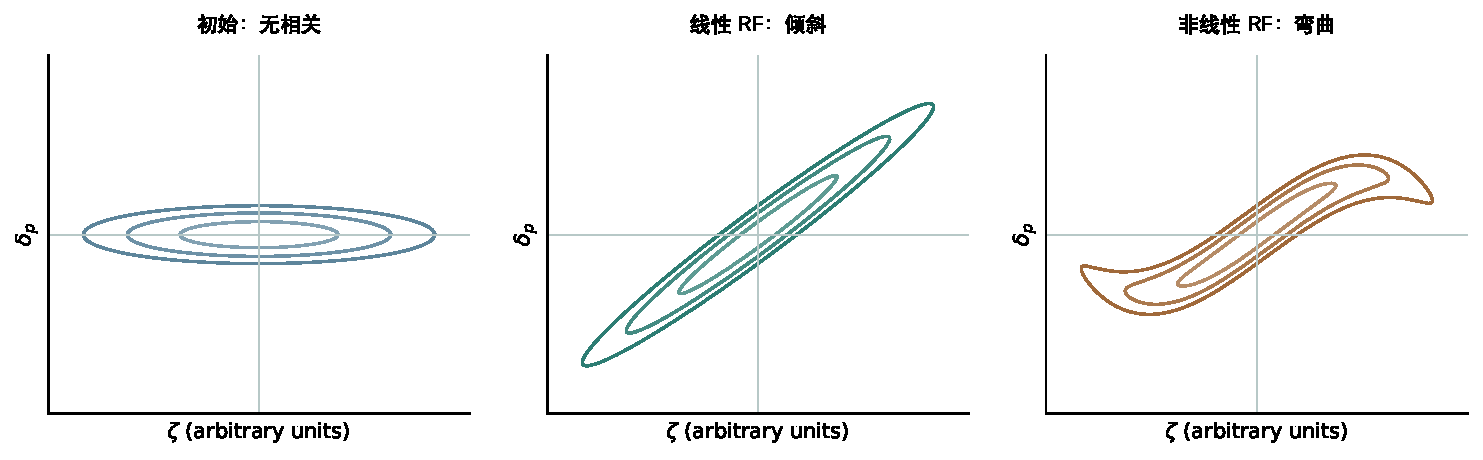
\includegraphics[width=.96\linewidth]{figures/phase_space.pdf}
\caption{统计概念示意，不是新模拟。线性剪切可以增加展宽而保留 RMS 面积；非线性弯曲可能增加线性拟合后的剩余厚度。}\end{figure}
严格说，$\sqrt{\det\Sigma}$ 是相空间面积的尺度；对于 $\mathbf u^T\Sigma^{-1}\mathbf u=1$ 的椭圆，其几何面积为 $\pi\sqrt{\det\Sigma}$。该椭圆也不代表所有粒子都在其中。

投影 RMS 发射度不是熵。无碰撞动力学可保留细粒度相空间体积，却由于非线性或跨方向投影改变 RMS 面积；不能把任何增长都叫代码耗散，也不能要求所有工况单调增长。
\source{式~\eqref{eq:residual} 由中心矩直接推导；\coderef{diagnostic}；既有闭合分析\ev{E05}。}

\subsection{漂移：没有外场也会改变尺寸}
固定参考能量的一阶纵向关系为
\begin{equation}
 \zeta'=\delta_p/\gamma^2,\qquad
 \binom{\zeta_2}{\delta_2}=\begin{pmatrix}1&L/\gamma^2\\0&1\end{pmatrix}\binom{\zeta_1}{\delta_1}.
\end{equation}
因此 $A_2=A_1+2LC_1/\gamma^2+L^2B_1/\gamma^4$。负相关束团可先压缩后展长；无初始 chirp 的有限展宽束团通常展长。RF 入口状态不能直接用最初的 300 $\mu$m 代替。

OCELOT 当前漂移保留二阶。独立质量壳自由飞行参考为
\begin{align}
 w&=\sqrt{1+2q/\beta+q^2-a^2-b^2},\\
 x_2&=x_1+La/w,\quad y_2=y_1+Lb/w,\\
 \tau_2&=\tau_1+L[(1/\beta+q)/w-1/\beta].
\end{align}
要求真实正能量、正向运动 $w>0$。二阶展开包含
\begin{equation}
 \Delta\tau=L\left[-\frac q{\beta^2\gamma^2}+\frac{a^2+b^2}{2\beta}
 +\frac{3q^2}{2\beta^3\gamma^2}\right]+O(3).
\end{equation}
它有角度飞行时间和动量非线性，AG 的约化一阶运动学不自动包含。细分步长不能把二阶截断模型变成精确自由飞行。
\source{\path{GPT模拟/transport_physics_note.md}、\path{validation/test_ocelot_transport.py}；\ev{E06}；原生坐标\cite{occoord}。}

\subsection{磁透镜：近轴硬边界聚焦}
螺线管强度 $k_s=eB_z/(2p_0)$ [m$^{-1}$]。近轴硬边界模型包含拉莫尔转动和聚焦；适当旋转坐标下有 $-k_s^2\sigma$ 型包络聚焦，有限面积提供 $M/\sigma^3$ 型展宽，SC 再加入集体作用。

OCELOT 正式磁透镜是\textbf{一阶 TransferMap}。独立检查使用二次横向 Hamiltonian 的矩阵指数。已安装版 Solenoid 的二阶张量缺必要磁刚度色差，不能因为支持 SecondTM 接口就称真二阶磁透镜。

AG 默认 \texttt{solenoid\_coupling=False}，证据围绕共享圆束和规定线性范围。一般非圆束、完整耦合、色差、真实端场和像差仍未全面验收。一阶参考动量的数学检查不证明强能散束团精度。
\source{\path{AG/external_forces.py}；\coderef{method}；传输 Note、\ev{E06}；官方元件架构\cite{ocelements}。}

\subsection{RF：同一有效模型，不同纵向近似}
当前是\textbf{固定参考、入口薄透镜、有效积分电压}。负电子电荷和腔极性吸收到相位约定。令 $k=2\pi f/c$，粒子侧扣除理论参考增益：
\begin{equation}
 g(\tau)=V_{\rm eff}[\sin(\phi-k\tau)-\sin\phi]\ [\mathrm{eV}],\qquad
 q^+=q^-+g(\tau)/(\beta E_{0,\mathrm{eV}}).
 \label{eq:rfsine}
\end{equation}
$V$ 用 V 输入，电子能量数值用 eV。不是扣样本均值，也没有更新共同加速参考。用 $\tau=-\zeta/\beta$ 线性化得
\begin{equation}
 \delta_p^+=\delta_p^-+H\zeta,\qquad
 H=\frac{V_{\rm eff}k\cos\phi}{\beta^3 E_{0,\mathrm{eV}}}.
 \label{eq:rfh}
\end{equation}
其中一个 $1/\beta$ 来自长度到到达时间相位转换，另两个来自能量到动量归一化。当前已修复旧公式缺失的转换因子；默认 $H\approx-17.8374$ m$^{-1}$。

AG 在同一状态作协方差变换：
\begin{equation}
 A^+=A^-,\quad C^+=C^-+HA,\quad
 B^+=B^-+2HC^-+H^2A,\quad D^+=D^-.
 \label{eq:rfcov}
\end{equation}
它应满足零强度恒等、$\pm H$ 可逆。粒子正弦曲率不必保留投影 RMS 的 $D$。对任意 $\delta^+=\delta+g(\zeta)$，中心矩给出
\begin{align}
 D^+-D^-={}&2[A\operatorname{Cov}(\delta,g)-C\operatorname{Cov}(\zeta,g)]\notag\\
 &+A\operatorname{Var}(g)-\operatorname{Cov}(\zeta,g)^2.
 \label{eq:nonlinearkick}
\end{align}
线性 $g=H\zeta$ 相消，正弦一般不相消。因此 RF 后面积不同可能是近似所致，需要独立参考判断，不能直接认定代码错误。

横向共同近似为 $K_\perp=-H/(2\gamma^2)$，$a^+=a^-+K_\perp x$，$b$ 同理；AG 更新包络斜率。它依赖轴对称、近轴、弱场近似恒速、积分端部场消失和穿腔横向位移近似不变。默认横向 RF 关闭。
\begin{plainbox}\textbf{腔长不是自动的有限场模型}\par
RF 的 22 mm 是几何占长，kick 在入口，body 按漂移。改变腔长不会自动计算真实轴向场或渡越因子。$V_{\rm eff}$ 已是含渡越效应的有效积分幅值，不能从 $V_{\rm eff}/L$ 推断设备峰值场。
\end{plainbox}
\source{\coderef{rfshared}、\coderef{rfag}；共同 RF Note；独立参考\ev{E03}；有效积分及 $\omega/v$ 关系\cite{franssen}。式~\eqref{eq:nonlinearkick} 是已有矩关系的代数展开。}

\subsection{SC：不是一块单独的外加元件}
空间电荷来自束团自身的电磁场，在各段传播中不断改变动量、chirp、尺寸和关联。改变物理 $Q$ 改变集体力；仅增加宏粒子 $N$ 应主要改变数值分辨率。AG 按高斯统计量求平均力与矩关联；OCELOT 从当前云求自洽近似场，保留更多非高斯结构，但有网格和有限步误差。
\source{高斯矩方程\cite{kelisani}；官方三维 SC\cite{ocsc}；两条路线的生产调用。}

\section{模型内部状态与数值算法}\label{sec:models}
\subsection{AG：F/G 配对与同一纵向状态}
对 $u=x,y,\zeta$ 定义中心化矩
\begin{equation}
 \sigma_u=\sqrt{\langle u^2\rangle},\quad\nu_u=\sigma_u',\quad
 \theta_u=\sqrt{\langle u'^2\rangle},\quad M_u=\sigma_u^2(\theta_u^2-\nu_u^2).
\end{equation}
固定参考下的结构是
\begin{equation}
 \sigma_u'=\nu_u,\quad\nu_u'=\frac{\theta_u^2-\nu_u^2}{\sigma_u}+F_u,\quad
 \theta_u'=G_u,\quad M_u'=2\sigma_u^2(\theta_uG_u-\nu_uF_u).
 \label{eq:fg}
\end{equation}
$F_u$ 是包络加速度项 [m$^{-1}$]，不是单电子 SI 力 [N]；$G_u$ 描述斜率分散。程序用配对面积式避免大项相消。纵向对应
\begin{equation}
 C=\gamma^2\sigma_\zeta\nu_\zeta,\quad B=\gamma^4\theta_\zeta^2,\quad
 D=\gamma^4M_\zeta,\quad\varepsilon_{n,p}=\beta\gamma^3\sqrt{M_\zeta}.
\end{equation}
只积分 $(\sigma_\zeta,\nu_\zeta,M_\zeta)$，其余纵向量由它推导；SC 与 RF 不再各算一套状态。内部活动向量共 12 项，含三尺寸、横向相关兼容量、三斜率、相关斜率、$\gamma$ 和三面积；\textbf{不是完整六维分布的 21 个独立协方差}。公开 history 保留前 12 列，再加两横向发射度，共 14 列，分段重建要传完整行。
\source{论文式 (3)、(6)--(7)、(15)--(20)\cite{kelisani}；纵向/横向 G Notes；\coderef{state}、\coderef{g}。}

\subsection{高斯 SC、九项系数与发射度的结构限制}
令 $k_x=\sigma_x/(\gamma\sigma_\zeta),k_y=\sigma_y/(\gamma\sigma_\zeta)$，
\begin{equation}
 f_b=\frac{e}{mc^2}\frac{N_e e}{8\pi\sqrt\pi\epsilon_0}\ [\mathrm m],\qquad\bar p_0=\beta\gamma.
\end{equation}
领先项例如 $F_x^{s,0}=f_b\alpha_x/(\beta^2\gamma^3\sigma_x\sigma_\zeta)$，
$F_\zeta^{s,0}=f_b\alpha_\zeta/(\beta^2\gamma^3\sigma_x\sigma_y)$。\textbf{正式计算还保留论文中含 $\theta,\nu$ 的修正项}；不能只用两个领先项代替生产公式。完整 F 在快照 \path{AG/beam_dynamics_6d.py::_space_charge_forces}，纵向摘录见\coderef{force}。

九个无量纲系数统一为
\begin{equation}
 I=C_\alpha\int_0^\infty t\prod_{j=x,y,z}(t^2+a_j^2)^{-p_j/2}dt,
 \qquad(a_x,a_y,a_z)=(k_x,k_y,1).
 \label{eq:alpha}
\end{equation}
$t$ 是无量纲积分变量，不是位置或到达时间。参数表见附录~\ref{app:alpha}。定义
\begin{equation}
 X=\frac{\nu_x\alpha_x}{\sigma_x\sigma_\zeta},\quad
 Y=\frac{\nu_y\alpha_y}{\sigma_y\sigma_\zeta},\quad
 Z=\frac{(1-\bar p_0^2)\nu_\zeta\alpha_\zeta}{\sigma_x\sigma_y},
\end{equation}
F/G 配对给出当前面积演化：
\begin{equation}
 \begin{pmatrix}M_x'\\M_y'\\M_\zeta'\end{pmatrix}
 =-\frac{2f_b}{\gamma}\begin{pmatrix}(3X+Y+Z)M_x\\(X+3Y+Z)M_y\\(X+Y+3Z)M_\zeta\end{pmatrix}.
 \label{eq:grates}
\end{equation}
Gx/Gy/Gz 都已存在，但该齐次方程不含任意非高斯非线性关联的全部面积生成机制。系数有限时 $M=0$ 保持为零，而非线性 kick 可把冷分布弯成有 RMS 投影面积的曲线。这是闭合限制，不能单靠重构修好。

均匀椭球选项内部力线性，SC 面积变化率为零。它适合对应分布/线性极限研究，不是为了拟合 PIC 而可任意替换的默认；理论来源为 Luiten 等\cite{luiten}。
\source{\coderef{g}；原论文 G 独立转写测试；\ev{E05} 的代数与旧云分析。}

\subsection{AG 积分与系数误差控制}
RK45 默认 rtol=$10^{-8}$、atol=$10^{-10}$；\texttt{n\_points} 只是输出采样预算。三面积以 $10^{-12}$ m$^2$ 缩放。积分检查 success、终点、有限值、正尺寸与非负面积。非法 RK45 试算阶段从未改变的已接受状态缩步，最多 32 次；不裁剪负束宽。此包装依赖已核对的 SciPy 状态提交顺序，升级应重新检查。

$\alpha$ 已从旧 $15\times15$ 截断表改为对数变量直接积分，每轴数值域 $[10^{-6},10^6]$，域外明确失败。16/32 点 Gauss--Legendre 比较，必要时 64/128 点；相对加阶目标 $5\times10^{-11}$，尾部另有解析界。F/G 共用入口，记录全部 RHS 请求。加阶差不是严格总误差界，数值域也不是物理适用域。
\source{\coderef{alpha}；$\alpha$ Note、\ev{E02}；独立 Carlson $R_D$ 定义\cite{scipyrd}。}

\subsection{OCELOT 的正式追踪与 SC 契约}
builder 按共享几何建立 lattice；不激活的有长度元件保留同长 Drift。用类对象请求实际方法并检查活动 \texttt{tms}，当前策略是 \texttt{drift\_second\_order\_solenoid\_linear\_v1}。不从字符串标签或 Twiss 路径推断真实追踪方法。

每次从有效配置生成云：$\sigma_\tau=\sigma_\zeta/\beta$，$\sigma_q=\beta\sigma_\delta$。位置 seed、动量 seed+1。有限云实际矩不等于名义高斯，比较应保留初态实测值。

无 SC 用 \path{tracking_step}，跨 RF 入口切步并补尾段。有 SC 用原生 \path{Navigator.get_next_step}：步起点处理已到达的 RF 入口，应用传输映射，再应用返回物理过程并取样。零长原生边界定位 RF 入口；SC 间隔、计数和覆盖仍由原生调度决定。

SC requested=True 时，导入、构造、attach、真实 apply 与 cathode--sample 覆盖失败必须报错；effective 由实际执行决定，不能因可选模块失败静默退成无 SC。requested=False 时可选 SC 不可用不应阻止无 SC 计算。
\source{\coderef{method}、\coderef{schedule}；\path{shared/sc_state.py} 与正式入口专项。}

\subsection{三维 PIC 的局部数学与近似}
实际链为：原生过面坐标 $\to$ 同一实验室时刻坐标 $\to$ 平均动量方向/共同 $\gamma$ 的束团系 $\to$ NGP 沉积 $\to$ FFT 自由空间卷积 $\to$ 差分/插值/boost $\to$ kick $\to$ 原生坐标。
\begin{equation}
 \nabla^2\Phi'=-\rho'/\epsilon_0,\qquad
 \Phi'(\bm r)=\frac1{4\pi\epsilon_0}\int\frac{\rho'(\bm r')}{|\bm r-\bm r'|}\,d^3r',\quad\bm E'=-\nabla\Phi'.
\end{equation}
自由空间不含导体壁、阴极镜像或真实腔体边界。当前共同速度近似的有效力与有限步冲量为
\begin{equation}
 \bm F_{\rm eff}=\bm E_\parallel+\bm E_\perp/\gamma_{\rm av}^2,\qquad
 \Delta(\bm P c)=(ds/\beta_{\rm ref})\bm F_{\rm eff},
\end{equation}
后式采用电子 eV、V/m、m 数值约定。它不是逐粒子精确连续 Lorentz 求解；固定参考时长可产生相对空间功的 $O(ds^2)$ 局部偏差，不能据此认定整线全局阶数。

球高斯独立参考来自 Gauss 定律：
\begin{equation}
 E_r(r)=\frac Q{4\pi\epsilon_0r^2}\left[\operatorname{erf}\!\left(\frac r{\sqrt2\sigma}\right)
 -\sqrt{\frac2\pi}\frac r\sigma e^{-r^2/(2\sigma^2)}\right].
\end{equation}
它分开检验场、kick 和坐标，不调用 AG 系数自证。正式初态为等权宏粒子；非等权云、大角度、强能散/压缩与导体边界尚未全面验收。
\source{官方 SC\cite{ocsc}；\path{GPT模拟/sc_local_physics_note.md}；\ev{E07}。}

\section{几何、事件与 GUI 运行过程}\label{sec:gui}
\subsection{默认束线与元件移动规则}
\begin{figure}[H]\centering
\begin{tikzpicture}[x=.018cm,y=1cm,font=\small,>=Latex]
\draw[->] (0,0)--(790,0) node[right] {$s$};
\fill[accent!20] (100,-.16) rectangle (160,.16);\fill[warm!35] (400,-.16) rectangle (422,.16);
\foreach \p in {0,100,160,400,422,777}{\draw (\p,-.2)--(\p,.2);}
\node[above=3mm] at (130,0) {磁透镜};\node[above=3mm] at (411,0) {RF};\node[above=3mm] at (777,0) {样品};
\foreach \p/\y in {0/-.6,100/-.6,160/-1,400/-.6,422/-1,777/-.6}{\node at (\p,\y) {\p};}
\node at (45,.5) {漂移};\node at (280,.5) {漂移};\node at (595,.5) {漂移};
\node[anchor=east] at (777,-1.5) {刻度 mm；RF kick 在 400 mm 入口};
\end{tikzpicture}
\caption{0--100、160--400、422--777 mm 为显式漂移；RF 占长 22 mm。}
\end{figure}
共同几何校验要求入口等于前面长度累计值，sample 是唯一末端零长标记，束线为正，诊断面在覆盖内。只容许 64 ULP 累加舍入，不允许真实间隙/重叠。移动腔体须显式调整邻段漂移，不自动移动样品；关闭物理作用仍保留几何占长。

GUI 支持表格增删/修改元件，没有拖拽自动重排。低层调用者手建 lattice 直接调用 \texttt{run\_beamline} 时，仍须自行保证与配置一致。
\source{\coderef{geometry}；\path{shared/geometry_contract.md}；几何专项测试和 2026-10-22 报告。}

\subsection{GUI 怎样运行并保存一次计算}
工作配置提交本地服务，预检后冻结为任务输入。队列顺序启动 worker，每次调用一个正式 driver。目录保存配置、job、日志、进度/错误和结果；成功还须确认到达样品面。
\begin{figure}[H]\centering
\begin{tikzpicture}[>=Latex,node distance=6mm,
 box/.style={draw=accent!50,rounded corners,align=center,text width=29mm,minimum height=10mm,font=\small}]
\node[box,fill=pale] (e) {工作配置\\可编辑};\node[box,right=of e] (q) {校验/冻结\\queued};
\node[box,right=of q] (r) {真实 worker\\running};\node[box,right=of r,fill=pale] (c) {终点/结果完整\\complete};
\node[box,below=of r,text width=68mm] (f) {failed / cancelled / timeout / interrupted\\分别记录，不冒充成功};
\draw[->] (e)--(q);\draw[->] (q)--(r);\draw[->] (r)--(c);\draw[->] (r)--(f);
\end{tikzpicture}\caption{重启后把未结束任务标为 interrupted，不自动重跑。}\end{figure}

配置指纹避免不同配置曲线被当成同一比较。AG 进度按完成分段更新，OCELOT 按真实诊断位置更新。导出图保留单位/图例，ZIP 保留输入/日志。服务只监听 \texttt{127.0.0.1:8765}，默认数据 \path{gui_runs/} 不覆盖共享默认；当前没有多人服务、自动优化或真实装置控制。
\source{\coderef{worker}；\path{gui/server.py}、\path{web/app.js}；工程验收\ev{E09}。}

\subsection{Windows 工程复核：已修复与尚未实测}
三个 .bat、依赖 pin 与 \texttt{platform\_compat} 提供跨平台入口。2026-10-25 保存记录是 38 通过、6 个 Windows 原生项跳过；本轮补查失效路径，发现“已有测试通过”仍遗漏以下问题。

旧实现把 \texttt{taskkill} 非零退出当成功，强停后又无限等待；Win32 HANDLE 没有显式函数签名，访问/等待错误被当成父进程已死；监视线程写错误文件失败时不能保证退出。这些属于工程缺陷，不能归为物理模型差异。

当前改为检查停止命令退出码、句柄兜底和有限等待；无法确认退出则暂停队列。Windows 父进程句柄在启动时打开并保留，明确区分退出与 API 失败。取消宽限后升级强停；超时参数必须是有限正数。安装器拒绝非 CPython 3.12 x64 的既有环境，脚本禁用延迟展开并检查目录切换。

最终单元/契约测试 52 项中 46 通过、6 个 Windows 原生项跳过。真实 GUI 端到端 4 项通过：AG/OCELOT 各一条 10 mm 无 SC、含磁透镜与 RF 的正式短例，以及进入 AG 积分后的取消、关闭服务清理。两轮合计 4 条完整短轨迹、4 次中断 SC 调用；没有新增完整 SC 精度研究。

\textbf{这些证据仍来自 macOS。}Windows 的 Win32 调用、.bat 双击、真实控制台/杀毒/文件占用行为未实测；mock 只能核对接口和失效处理。每 2 秒是父进程轮询间隔，不是所有情况下 2 秒内清理的保证。
\source{旧记录\ev{E10}；本轮报告、测试账本及日志\ev{E11}；\coderef{platform}；Python/Win32 官方接口\cite{pyctypes,winprocess,winwait}。}

\section{已有证据究竟支持什么}\label{sec:evidence}
\subsection{工程、数学、数值和设备分开判断}
工程看真实配置/事件/终点/保存；数学看解析解、独立积分和必要恒等式；数值看指定工况的分辨率/统计误差；设备对应看校准和测量。两模型相近、某个测试 PASS 或漂亮曲线，都不能单独完成四者的论证。本文借用 V\&V/UQ 分层思想，NIST 来源是 CFD 方法学，不是 UED 专用精度标准\cite{nist}。

\subsection{已修复的状态和系数问题}
旧 AG 曾只演化包络却未一致更新纵向相关/展宽，使零强度 RF 改变状态。现在同一独立状态和配对 G 已修复此类问题。零 RF、$\pm H$、矩约束、论文 G 独立转写和正式保存链已有针对性检查；不等于高斯闭合全域精确。

2026-10-22 的 $\alpha$ 九系数在 248 点对独立自适应积分最大相对差约 $7.8\times10^{-15}$；55 位原变量积分 8 锚点约 $6\times10^{-15}$。默认 AG SC 轨迹记录 4314 次请求、最大比例约 379.097，截断为零。这是有限点实测，不是连续域严格机器误差保证。
\source{\ev{E01}、\ev{E02}；状态/G/$\alpha$ Notes。}

\subsection{RF 独立数学参考与线性化误差}
2026-10-24 固定 100 keV、30 kV、2.856 GHz、$\phi=3.1416$、$\sigma_\delta=10^{-4}$、$C=0$；SC/横向 RF/磁透镜关，对规定高斯入射作高精度积分与特征函数互证。两模型正式 CLI 各三例，共六条历史轨迹。
\begin{table}[H]\centering\small
\begin{tabular}{rrrr}\toprule
入射 $\sigma_\zeta$ & RMS 相位跨度 & 展宽线性/正弦差 & 发射度线性/正弦差 \\ \midrule
30 $\mu$m & 0.003276 rad & $+0.000518\%$ & 约 $-2.75\times10^{-8}\%$ \\
300 $\mu$m & 0.03276 rad & $+0.05363\%$ & $-0.02743\%$ \\
3000 $\mu$m & 0.3276 rad & $+5.410\%$ & $-95.50\%$ \\
\bottomrule\end{tabular}
\caption{差定义为 $X_{\rm linear}/X_{\rm sine}-1$；理想高斯与相同常量，来源\ev{E03}。}
\end{table}
相位跨度大时，面积的线性近似误差可比展宽明显得多。第三例是压力测试，不能证明强调制一阶动量适配有效。这些规定入射不是默认整线的实际 RF 入射。

当时无 SC RF 快照与 SC$\times$纵向 RF 四组合的八条基础整线已完成，见\ev{E04}。它定位差异在哪段出现，但采用旧传输方法；方法修正后不能直接移作当前 SC 精度结论。

\subsection{为什么保留 AG，却限制发射度定量使用}
既有推导得到式~\eqref{eq:grates}；旧方法下 RF 入射云的高阶拟合显示有线性相关之外的结构。这支持低阶高斯闭合存在限制，不足以证明全部差异都只有一个原因。

AG 可继续用于快速扫描、趋势和可解释分析；对已审查 SC 类工况，\textbf{不单独把其纵向发射度/增长当已验证定量预测}。需要束质结论时用有数值控制的粒子结果及独立参考。只有明确研究问题受阻时才考虑新闭合，不以升级模型作为 GUI 前置条件。
\source{零新增轨迹的闭合推导与冻结云分析\ev{E05}；旧数值保留原方法含义。}

\subsection{OCELOT 局部 SC 检查与代表整线研究}
2026-10-25 的 45 项局部数学/执行检查覆盖独立高斯场、Poisson、坐标、规定场 kick、零路径/零场及 2 mm 正式短例。短例 100 keV/100 fC、N4000、$33^3$、dz0.5 mm、RF关，4次真实 SC。所选球高斯点的直接 Poisson 场最大误差，$33^3/63^3$ 约 3.82\%/1.10\%；这是特定源与点，不是整线误差界。局部未发现需补的当前公式实现，不等于所有工况精度已证明。
\source{\ev{E07}；当前 SC Note；官方算法\cite{ocsc}。}

O3 使用当前漂移二阶/磁透镜一阶，100 keV/100 fC，85/300 $\mu$m、$\sigma_\delta=10^{-4}$、$\varepsilon_{nx/y}=0.08\mmemit$，777 mm 束线，SC/纵向 RF 开、横向 RF 关。
\begin{table}[H]\centering\small
\begin{tabular}{lrrrrl}\toprule
设置 & N & 网格 & dz/mm & seed & 状态 \\ \midrule
baseline & 50000 & $63^3$ & 1 & 42 & 到样品 \\
N100k & 100000 & $63^3$ & 1 & 42 & 到样品 \\
mesh95 & 50000 & $95^3$ & 1 & 42 & 到样品 \\
dz\_half & 50000 & $63^3$ & 0.5 & 42 & 到样品 \\
seed43 & 50000 & $63^3$ & 1 & 43 & 到样品 \\
combined & 100000 & $95^3$ & 0.5 & 42 & 累计预算结束 \\
\bottomrule\end{tabular}
\caption{最多 6 尝试，单条 1800 s、累计 5400 s；5 条完整，联合加密未完成。}
\end{table}
\begin{table}[H]\centering\small
\begin{tabular}{lrr}\toprule
样品面观测量 & 基准值 & 已完成控制相对基准最大绝对变化 \\ \midrule
$\sigma_x$ [$\mu$m] & 2558.213 & 0.47467\% \\
$\sigma_y$ [$\mu$m] & 2551.976 & 0.31542\% \\
$\sigma_\zeta$ [$\mu$m] & 2048.323 & 0.084046\% \\
$h$ [m$^{-1}$] & 5.129814 & 0.0070627\% \\
$\sigma_\delta$ [$10^{-3}$] & 10.51016 & 0.086636\% \\
$\varepsilon_{nx}$ [$\mmemit$] & 0.1306952 & 1.0949\% \\
$\varepsilon_{ny}$ [$\mmemit$] & 0.1289053 & 0.21727\% \\
$\varepsilon_{n,p}$ [$\mmemit$] & 0.3165068 & 1.7982\% \\
\bottomrule\end{tabular}
\caption{直接提取 E08 保存结果。最后一列是有限设置变化幅度，不是误差上界或置信区间。}
\end{table}

这组基准轨迹在保存的离散样点中，约498 mm处束长最短，为22.826 $\mu$m，之后再次展长，到777 mm样品面为2048.823 $\mu$m。因此“样品束长比初态大”不等于RF没有产生压缩；本例样品面处在已记录压缩点之后。498 mm只是采样最小值，不是精确束腰定位，也不是已优化设备性能。

完成云独立重算共同矩最大相对差约 $1.63\times10^{-12}$，这是保存/诊断一致性，不是物理精度。联合加密最后进度 285.5 mm，未到 RF；仅初态/配置/进度，没有样品 JSON 或该进度的粒子云，不能作为更精确真值。

两层分辨率、两个 seed 和未完成联合加密只支持\textbf{有限设置变化幅度}，不是完整收敛、置信区间或误差上界。共享默认仍是 SC关/dz5 mm，不能自动继承本轮 1/0.5 mm SC 结论。
\source{\ev{E08} 的 analysis、specs、ledger、termination、saved\_verification；表中数值自动读取保存 JSON。}

\subsection{当前测试入口的日期边界}
源码 \texttt{run\_all.py} 现注册\textbf{12组}：\path{config_schema}、drift、solenoid、rf、\path{full_beamline}、\path{gpt_route}、\path{runner_contract}、\path{ag_longitudinal}、\path{ag_transverse_g}、\path{diagnostics_rf}、\path{alpha_numerics}、\path{ocelot_transport}。旧说明的11组是版本/日期差异。

最近完整 suite 记录为2026-10-22的11组；10月25日是方法/SC专项，\textbf{没有据此宣称当前12组整套复跑通过}。GUI、Windows和其他专项也不全包含其中。该脚本会写报告与检查点，本次文档整理未运行它。
\source{当前注册表、\path{PROJECT_STATUS.md} 日期记录、\ev{E06}--\ev{E11}。}

\section{尚存在的问题与后续顺序}\label{sec:issues}
\subsection{当前问题总表}
\begin{longtable}{P{30mm}P{33mm}P{87mm}}\toprule
事项 & 当前判断 & 影响/剩余工作 \\ \midrule\endhead
正式路线重复 & 相关路径已合并 & 每模型一套 driver；旧原型仍需标签，不等于所有旧脚本被验收。\\
AG 电荷、纵向状态 & 已针对性修复 & $N_e=Q/e$、同一状态、Gz与零RF已查；不要把旧 bug继续列成未修。\\
Gx/Gy与发射度 & 已恢复，模型有限 & 不再强制固定；高阶/非高斯/一般耦合未完整保留。\\
$\alpha$ 截断/精度 & 数值旧问题已解决 & 直接积分、域外失败；物理适用域不由数值域保证。\\
RF因子、开关、位置 & 已有修复与检查 & 固定参考薄透镜内使用；真实有限场/共同加速/设备标定开放。\\
OCELOT活动方法 & 已修静默回退 & 漂移二阶，磁透镜一阶；色差、端场与高阶未纳入。\\
SC局部数学 & 限域通过 & 共同速度/自由空间/等权云；其他边界待用途驱动研究。\\
数值精度 & 有限研究已结束 & O3非全收敛；新阈值/工况应先写卡片，不无限追加扫描。\\
常量一致性 & ppm差异保留 & AG静能、共享511 keV和RF归一化有差；不能解释百分比/倍数级SC差。\\
输出事件侧 & 已知语义边界 & RF在s=0时AG起点可为RF后、粒子为RF前；需事件快照。\\
配置全量schema & 部分覆盖 & 几何集中、GUI有数值检查；CLI/API全字段组合验收未集中完成。\\
环境与Windows & pin已加入，实机待验 & 可用轮子不等于干净环境已安装；Windows双路线和清理行为缺实测。\\
文档漂移 & 仍存在 & 旧HEAD/路径/远端、旧RF句子、组数和方法需按日期读；本说明以快照为准。\\
全枪/样品/探测器 & 未建模，非当前漏洞 & 缺对应输入，不作为第一版GUI的前置条件。\\
\bottomrule\end{longtable}
这不是“漏洞已穷尽”的承诺。旧原型和第三方库所有功能未逐行验收。\texttt{AI\_HANDOFF}顶部仍有旧HEAD/远端等信息，需结合最新段落与实际Git；某项实现已修不能扩大成全项目物理认证。
\source{当前源码、Notes、状态表及\ev{E01}--\ev{E11}，范围按上一节解释。}

\subsection{整体 roadmap：先稳定使用，按问题提高精度}
\begin{plainbox}\textbf{下一阶段中心目标}\par
把已有物理方案变成可编辑、可运行、可导出、可复核的工具。保留已知模型边界，不以引入新模型为收尾条件。每次新计算必须有明确问题和可结束的预算。
\end{plainbox}
\begin{longtable}{P{10mm}P{39mm}P{49mm}P{52mm}}\toprule
顺序 & 工作 & 原因 & 完成条件 \\ \midrule\endhead
1 & Windows原生工程验收 & 兼容实现刚加入，缺真实平台证据 & 干净安装；双路线各一短例；运行中取消/超时/关服务，保留退出码和日志。\\
2 & 常用工况和GUI范围标签 & 防止所有可调参数都被误读为精度已证 & 固定输入、数值设置、观测量和证据版本；区分默认/探索/已研究。\\
3 & 同步当前状态与环境信息 & 旧组数、路径和HEAD易误导 & 单一当前入口、方法与依赖可查，原报告不覆盖。\\
4 & 按研究目标补最少控制 & O3仅是有限敏感性 & 先定参考、阈值和预算；能支持/不支持/证据不足都可结束。\\
5 & 有设备数据后标定 & 默认值不能证明设备对应 & RF电压/相位/作用面、磁场和入射束流可追溯；独立实验及不确定度。\\
按需 & 新闭合/有限场/真二阶磁透镜/全枪 & 都扩大研究范围 & 仅当现模型阻挡具体目标时立项，研究者裁定假设与标准。\\
\bottomrule\end{longtable}

每轮先用现有计算卡记录：问题、主要量、参考及资格、有效配置、$T$来源、预算/停止条件、版本/seed和输出。误差/余量定义一致时可用 $E+U\le T$ 支持目标，$E-U>T$ 不支持，其余证据不足。$U$需说明经验或统计属性，不能随意把相关项按独立方差相加。近零chirp/增长量用预定绝对尺度。

预测压缩先看实际面的束长/时宽/chirp；讨论束质同时看发射度总值和增长；讨论RF先取同面同事件侧前后状态。每一步目的应能用一句普通中文说明。
\source{当前状态中的判定规则、\path{CALCULATION_CARD_TEMPLATE.md}；一般V\&V/UQ背景\cite{nist}。}

\section{使用、维护与文档复现}\label{sec:use}
macOS 双击 \path{启动界面.command}。Windows 按现有说明先 \path{安装环境.bat}，再 \path{启动界面.bat}；Windows实机范围仍如前述。手动命令：
\begin{Verbatim}[numbers=none]
python -X utf8 run_gui.py --open
python -X utf8 run_gui.py --port 8766 --data-dir "my runs" --timeout 1800
\end{Verbatim}
先预检，再选模型。默认SC关；开启后明确数值设置和effective/覆盖。PyPI发行名是\texttt{ocelot-collab}，导入名是\texttt{ocelot}。OCELOT CLI step1--3均无SC能力，step4才允许继承配置启用；GUI调用full API，按保存配置决定SC。

输入错误先查params/geometry/run\_contract；RF查共同模块与两调用点；AG状态查longitudinal\_state和完整14列重建；SC不生效先查请求/有效/次数/覆盖；输出差异先查单位、坐标、实际面与事件侧。工程修复最小验证；物理/数值变更更新Note与原因，不放宽阈值、不覆盖旧基线。

本LaTeX项目独立目录包含图、文献、代码与证据。可用XeLaTeX编译，再通过构建脚本补内嵌中文字符映射，以改善跨阅读器搜索/复制；后处理不改公式或版面：
\begin{Verbatim}[numbers=none]
python build_pdf.py
\end{Verbatim}
构建需要XeLaTeX、latexmk和Python的pypdf，不需要在线文献检索、BibTeX或OCELOT。Fandol随TeX发行版提供，等宽字体和字符映射随附许可。\texttt{prepare.py}会重新捕获当前仓库，不要随手重跑覆盖归档；\texttt{make\_figures.py}只画概念图并读旧JSON，不调用driver。

完整相关源码在\path{source_snapshot/}、逐文件哈希在\path{source_manifest.json}。附件便于定位，不是包含全部历史文件和运行环境的独立软件发行包；正式计算仍从项目根目录启动。大粒子云未复制，按证据清单查原目录。
